\documentclass[11pt, oneside]{article}   	% use "amsart" instead of "article" for AMSLaTeX format
%\usepackage{geometry}                		% See geometry.pdf to learn the layout options. There are lots.
%\geometry{letterpaper}                   		% ... or a4paper or a5paper or ... 
%\geometry{landscape}                		% Activate for rotated page geometry
%\usepackage[parfill]{parskip}    		% Activate to begin paragraphs with an empty line rather than an indent

\usepackage{geometry}
 \geometry{
 a4paper,
 total={170mm,257mm},
 left=20mm,
 top=20mm,
 bottom=20mm,
 }

\usepackage{graphicx}				% Use pdf, png, jpg, or eps§ with pdflatex; use eps in DVI mode
								% TeX will automatically convert eps --> pdf in pdflatex		
\usepackage{amssymb}
\usepackage{amsmath}
\usepackage{fancyhdr}
\usepackage[utf8]{inputenc}
\usepackage[english]{babel}
\usepackage{enumerate}
\usepackage{arcs}
\usepackage{cancel}
\usepackage{xfrac}
\usepackage{tikz}
\usepackage{array}
\usepackage{tabularx}

%SetFonts

%SetFonts

\usepackage[inline]{asymptote}


\pagestyle{fancy}
\fancyhf{}
%\rhead{Teacher David @ 18601688612}
\lhead{\leftmark}
\rfoot{\thepage}


\title{Math Notes}
\author{Peter He}
%\date{}							% Activate to display a given date or no date

\begin{document}
\maketitle




\section{Linear Functions}
\subsection{$y=kx$}
\begin{enumerate}
%\renewcommand{\labelenumi}{1.\arabic{enumi}}

\item $k\ne0$.
\item The line passes through the fixed point $(0,0)$.
\item $k$ is the gradient of the line.
\item If the line passes through another point $(a,b)$, then $k=\frac{b-0}{a-0}=\frac{b}{a}$, and therfore, $y=\frac{b}{a} x$.
\item If we move the line along the $y$-axis up for $b$ units, we will get another function $y=kx+b$. 
\end{enumerate}

\begin{center}
\begin{tikzpicture}[scale=0.7]

\draw[blue] (-1,-2) -- (2,4);
\draw[red] (-1,0) -- (2,6);
\draw[->,thick] (-3,0) -- (3,0);
\draw[->,thick] (0,-3) -- (0,3);
\filldraw(1,2)circle(1pt);

\coordinate [label=below:$x$] (x) at (3,0);
\coordinate [label=left:$y$] (y) at (0,3);
\coordinate [label=right:{$(a, b)$}] (a) at (1,2);
\coordinate [label=below:{$y=kx$}] (k) at (3.5,4);
\coordinate [label=below:{$y=kx+b$}] (l) at (3.5,6);


\end{tikzpicture}
\end{center}



\subsection{$y=kx+b$}
\begin{enumerate}


\item If $k>0$, the line is increasing; if $k<0$, the line is decreasing.
\item The line intersects with the $y$-axis at point $(0,b)$.
\item Point Slope Form: If the slope is $k$, and the line passes through point $(x_0,y_0)$, then \[y=k(x-x_0)+y_0\].
\item Any two distinctive points $(x_1,y_1), (x_2,y_2)$ determine a line, where $k=\frac{y_2-y_1}{x_2-x_1}$ and \[y=\frac{y_2-y_1}{x_2-x_1}(x-x_1)+y_1\] or  \[y=\frac{y_2-y_1}{x_2-x_1}(x-x_2)+y_2\]
\item The derivative of $y$ at ay point on the line is $k$.
\end{enumerate}


\section{Quadratic Function}
Given Quadratic Function: $y=ax^2+bx+c, a \ne 0$
we can turn the Function into the Vertex Form.
\begin{align*}
y&=ax^2+bx+c\\
&=a\left(x^2+\frac{b}{a}x+\frac{c}{a}\right)\\
&=a\left[(x+\frac{b}{2a})^2-\frac{b^2}{4a^2}+\frac{4ac}{4a^2}\right]\\
&=a\left(x+\frac{b}{2a}\right)^2+\frac{4ac-b^2}{4a}
\end{align*}
The vertex of the parabola of function $y=ax^2+bx+c$ is $(-\frac{b}{2a},\frac{4ac-b^2}{4a})$.\\
The axis of symmetry  for this function is $x=-\frac{b}{2a}$.

\subsection{Intersections with $x$-axis}
If the parabola intersects with the $x$-axis, then at the intersection points we have $y=0$. Therefore, solving the equation $ax^2+bx+c=0$ discloses the coordinates of the intersection points. According to the vertex form, the equation becomes 
\begin{align*} 
&a\left(x+\frac{b}{2a}\right)^2+\frac{4ac-b^2}{4a}=0\\
\Rightarrow \quad &\left(x+\frac{b}{2a}\right)^2=\frac{b^2-4ac}{4a^2}\\
\Rightarrow \quad &x+\frac{b}{2a}=\frac{\pm \sqrt{b^2-4ac}}{2a}\\
\Rightarrow \quad &x=\frac{-b\pm \sqrt{b^2-4ac}}{2a}\\
\end{align*}
Finally, the intersection points are
\[(\frac{-b - \sqrt{b^2-4ac}}{2a},0), \quad (\frac{-b + \sqrt{b^2-4ac}}{2a},0) .\]
Apparently, if $b^2-4ac=0$, there is only one intersection point $(-\frac{b}{2a},0)$;
If $b^2-4ac<0$, there's no intersection point (The parabola doesn't intersect with the $x$-axis).
\begin{figure}
\centering
\begin{tikzpicture}[scale=0.7]

\draw[thick,blue] (-1,3) parabola bend (2,-1.5) (5,3);
\draw[->,thick] (-2,0) -- (6,0);
\draw[->,thick] (0,-3) -- (0,4);
\draw [dashed](2,3) -- (2,-3);
\draw (0.29,0) -- (0.29,0.5);
\draw (3.71,0) -- (3.71,0.5);

\draw[<-](2,0.4) --(2.6,0.4);
\draw[->](3.11,0.4) --(3.71,0.4);


\coordinate [label=above:$d$] (d) at (2.85,0);
\coordinate [label=below:$x$] (x) at (6,0);
\coordinate [label=left:$y$] (y) at (0,4);
\end{tikzpicture}
\caption{Parabola of a quadratic function.}
\label{fig:parabola}
\end{figure}

Given quadratic function $f(x)$, if its vertex is $(2,-1.5)$, and it intersects the $x$-axis at points $(1,0), (3,0)$, 
we can find out the quadratic expression of $f(x)$ via two methods.

\begin{itemize}
\item Method 1: Using the vertex form \\
Since the vertex is $(2,-1.5)$, $f(x)=a(x-2)^2-1.5$. Notice that point $(1,0)$ is on the curve, we have $f(1)=a(-1)^2-1.5 = 0, a=1.5$.
\item Method 2: Giving the intersection points are $(1,0), (3,0)$, we have $f(x)=a(x-3)(x-1)$.\\ Since the vertex is $(2,-1.5)$, we have $f(2)=a(2-3)(2-1)=-1.5, a =1.5$.
\end{itemize}
It seems like Method 1 requires merely 2 points to determine the parabola, and Method 2 requires 3 points in order to solve the parabola. However, the two Methods both require the same amount of information to determine the parabola. This is because we have the vertex $(2,-1.5)$, which helps determine the third point whenever another point is provided. For example, if we are only given one intersection point (1,0), we can know that another intersection point is (3,0) as they are symmetrical. If we are not given the vertex we need at least three different points to determine the parabola.

\subsection{Solving Quadratic Equation With Factorization}
When $f(x)=0$, the parabola intersects with the $x$-axis. To find out the intersecting points, we need to solve the equation $ax^2+bx+c=0$. There are many ways to solve quadratic equations. The vertex form, as we introduced in the previous section, is equivalent to completing square. In this section we introduce the method of factorization.  
Given equation $5x^2 + 7x -6=0$, it can be factorized as 
\[(5x-3)(x+2)=0\]
Once the equation gets factorized in the above form, its straightforward to get the roots by making either $5x-3=0$ or $x+2=0$.

The factorization method is essentially factorizing the coefficients of the first term and the third term, e.g. , 5 and $-6$ in the above example. We use a cross multiplication diagram to explain the process, as illustrated in Figure \ref{fig:factorization}. We factorize 5 into $5\times 1$ and put factors 5 and 1 into squares $A$ and $B$, and factorize $-6$ into $-3\times 2$ and put the factors $-3$ and 2 into squares $C$ and $D$. We cross multiply $AD$ and $BC$ such that $AD+BC=7$. We complete the factorization and get $(5x-3)(x+2)=0$.

\begin{figure}
\centering 
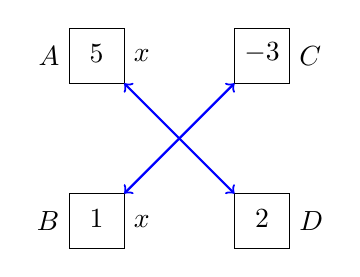
\begin{tikzpicture} [scale=0.7]

\draw (0,0) -- (0,1) -- (1,1) -- (1,0) -- cycle; 
\draw (3,0) -- (3,1) -- (4,1) -- (4,0) -- cycle; 
\draw (0,3) -- (0,4) -- (1,4) -- (1,3) -- cycle; 
\draw (3,3) -- (3,4) -- (4,4) -- (4,3) -- cycle; 

\draw [<->, blue, thick] (1,3)--(3,1);
\draw [<->, blue, thick] (1,1)--(3,3);

\coordinate [label=left:$A$](a) at(0, 3.5);
\coordinate [label=left:$B$](b) at(0, 0.5);
\coordinate [label=right:$C$](c) at(4, 3.5);
\coordinate [label=right:$D$](d) at(4, 0.5);

\coordinate [label=$5$](a1) at(0.5, 3.2);
\coordinate [label=$1$](b1) at(0.5, 0.2);
\coordinate [label=$-3$](c1) at(3.5, 3.2);
\coordinate [label=$2$](d1) at(3.5, 0.2);

\coordinate [label=right:$x$](a2) at(1, 3.5);
\coordinate [label=right:$x$](b2) at(1, 0.5);

\end{tikzpicture}
\caption{Factorization of $5x^2 + 7x -6$}
\label{fig:factorization}
\end{figure}


\subsection{Vieta's Formula}
Suppose the equation has two roots: $x_1, x_2$, then the equation can be written as
\[a(x-x_1)(x-x_2)=0.\]
Expanding the left hand side of the above equation, 
\[ax^2 - a(x_1 + x_2)x + ax_1 x_2 = 0.\]

The above equation implies that $b = -a(x_1 + x_2), c = ax_1 x_2$. Therefore the relationship between roots and coefficients is 



\[x_1 + x_2= -\frac{b}{a}, \quad  x_1 x_2 = \frac{c}{a}.\]
This is known as Vieta's Formula.

The Vieta's formula for cubic equation is stated as the following. Given cubic equation $ax^3+bx^2+cx+d=0$ with three roots, $\alpha, \beta, \gamma$, we have 
\begin{align*}
\alpha + \beta + \gamma &= (-1)^1 \cdot \frac{b}{a} = -\frac{b}{a}\\
\alpha\beta + \alpha\gamma + \beta\gamma &= (-1)^2 \cdot \frac{c}{a} = \frac{c}{a}\\
\alpha\beta\gamma &= (-1)^3 \cdot \frac{d}{a} = -\frac{d}{a}
\end{align*}
We can see that the power of $-1$ equals to the number of elements in each term of the left hand side in the equation. For example, in the second equation, each term has 2 elements, the right hand side therefore is $(-1)^2 \cdot \frac{c}{a}$.

In fact, the above three equations are the elementary symmetric polynomials of $\alpha, \beta, $ and $\gamma$. We will discuss the symmetric polynomials later.

\subsection{Another Way to solve quadratic equations}
Since solving the quadratic equations $ax^2+bx+c=0$ is equivalent to finding the intersection points to the $x$-axis for quadratic function $f(x)=ax^2+bx+c$, we can use the following method to solve quadratic equations.


The key to this method is to find  the distance $d$ from one of the intersection points to the axis of symmetry of the function, as illustrated in Figure~\ref{fig:parabola}.

Given equation $\frac{x^2}{2}-2x+\frac{1}{2}=0$, the axis of symmetry is $x=2$. Assume the two roots are $x_1, x_2$, we then have \[x_1=2-d, \quad x_2= 2+d.\]

According to \emph{Vieta's Formula}, $x_1 \cdot x_2= \frac{\frac{1}{2}}{\frac{1}{2}}=1$, we have 
\begin{align*}
&(2-d)(2+d)=x_1 \cdot x_2 =1\\
\Rightarrow\quad&2^2-d^2=1\\
\Rightarrow\quad&d^2=2^2-1=3\\
\Rightarrow\quad&d=\sqrt{3}\\
\Rightarrow\quad&x_1=2-d=2-\sqrt{3},\quad x_2=2+d=2+\sqrt{3}.
\end{align*}

This method is recommended by math Professor Po-Shen Loh from CMU(Carnegie Mellon University).

\newpage
\subsection{Symmetric Polynomials}
A symmetric polynomial is a polynomial where if you switch any pair of variables, it remains the same.
For example, $x^2+y^2-3xy$ is a symmetric polynomial. If we switch $x$ and $y$, it becomes $y^2 + x ^2 - 3yx$, which is the same as the original polynomial. Symmetric polynomials are closely related to Vieta's formula, and Newton's identities.

Given a problem where $x=2-\sqrt{3}, y=2+\sqrt{3}$, find $x^3 + y^3$. One way to solve this problem is to calculate $(2-\sqrt{3})^3$ and $(2+\sqrt{3})^3$, and its very tedious in calculation. A smarter way is to manipulate 
\[x^3+y^3=(x+y)(x^2+y^2-xy)=(x+y)((x+y)^2-3xy)=4(4^2-3)=52,\]
since it is quite easy to calculate $x+y=4$ and $xy=1$.

But how do you know that such manipulation will be an easier way to solve the problem?

Because we know the fundamental theorem of symmetric polynomials : every symmetrical polynomial can be expressed by elementary symmetric polynomials. 
 
 \subsection{Elementary Symmetric Polynomials}
 Elementary Symmetric Polynomials are the building blocks for all symmetric polynomials. Suppose there are $n$ different number of variables $x_1, x_2, \cdots, x_n$, we define the $n$ elementary symmetric polynomials as $e_1, e_2, \cdots, e_n$:
 \begin{align*}
 e_1&= \sum_{i=1}^{n} x_i \\
 e_2&=\sum_{1\le i<j\le n}x_i x_j\\
 \vdots\\
 e_n&=x_1 x_2  \cdots x_n
 \end{align*}
 Given 2 variables $x$ and $y$, there are 2 elementary symmetric polynomials: 
 \[e_1=x+y, \quad e_2=xy.\]
 Given three variables,$x$, $y$ and $z$, there are three elementary symmetric polynomials:
  \[e_1=x+y+z, \quad e_2=xy+xz+yz, \quad e_3=xyz.\]
  For symmetric polynomial $x^2+y^2-\frac{2}{xy}$, it can be expressed as 
  \[x^2+y^2-\frac{2}{xy} = (x+y)^2-2xy-\frac{2}{xy} ; \]
  For symmetric polynomial $\frac{1}{x^2} + \frac{1}{y^2} + \frac{1}{z^2}$, it can be expressed as:
  \[\frac{1}{x^2} + \frac{1}{y^2} + \frac{1}{z^2}=\frac{y^2 z^2+x^2 z^2+x^2 y^2}{x^2 y^2 z^2}=\frac{(xy+xz+yz)^2-2xyz(x+y+z)}{(xyz)^2}\]
  
  \subsection{Vieta's Formula ans Symmetry}
  Given equation $3x^3+2x^2+x-5=0$ with three roots $\alpha$, $\beta$, and $\gamma$, find the value of expression $\frac{1}{\alpha^2}+\frac{1}{\beta^2}+\frac{1}{\gamma^2}$. According to Vieta's formula, 
  \[\alpha+\beta+\gamma= - \frac{2}{3}, \quad \alpha\beta + \alpha\gamma +\beta\gamma= \frac{1}{3}, \quad \alpha\beta\gamma = \frac{3}{5},\] and
  \[\frac{1}{\alpha^2}+\frac{1}{\beta^2}+\frac{1}{\gamma^2}=\frac{(\alpha\beta+\alpha\gamma+\beta\gamma)^2-2\alpha\beta\gamma(\alpha+\beta+\gamma)}{(\alpha\beta\gamma)^2}=\frac{(\frac{1}{3})^2-2(\frac{3}{5}(\frac{2}{-3}))}{(\frac{3}{5})^2}\]
  
\subsection{Derivative}
For quadratic function the derivatives at different points are usually different. For example, given $f(x)=\frac{3}{2}(x-2)^2-\frac{3}{2}=\frac{3}{2}x^2-6x+\frac{9}{2}$, its derivative function $f'(x)=3x-6$. This means the derivative varies following the change of $x$. We can get the derivative of $f(x)$ at point $(1,0)$ using the derivative function $f'(x)$ : $f'(1)=3-6=-3$. Therefore, it is easy to determine the tangent line passing through $(1,0)$: $y=-3(x-1)+0$. The perpendicular line passing through $(1,0)$: $y=\frac{1}{3}(x-1)+0$. 

To make it clear, the derivative of $kx^2$ is $2kx$, and the derivative of $kx$ is $k$.  Figure~\ref{fig:derivative} illustrates how to compute the derivative at $x_0$.
\begin{figure}
\centering
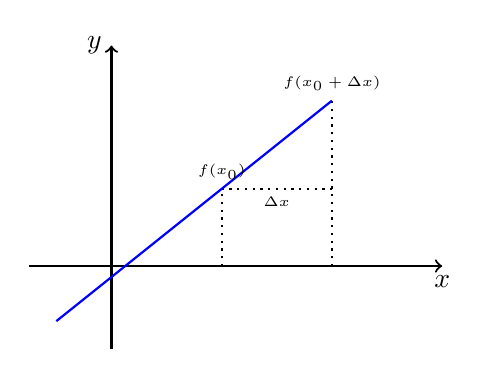
\begin{tikzpicture}[scale=0.7]


\draw[->,thick] (-1.5,0) -- (6,0);
\draw[->,thick] (0,-1.5) -- (0,4);
\draw [thick, dotted](2,0) -- (2,1.4);
\draw [thick, dotted] (4,0)--(4,3);
\draw [thick, dotted] (2,1.4)--(4,1.4);
\draw [thick, blue] (-1,-1) -- (4,3);

\coordinate [label=above:\tiny $f(x_0)$] (f1) at (2, 1.4);
\coordinate [label=above:\tiny $f(x_0+\Delta x)$] (f2) at (4, 3);

\coordinate [label=above:\tiny $\Delta x$] (d) at (3,0.9);
\coordinate [label=below:$x$] (x) at (6,0);
\coordinate [label=left:$y$] (y) at (0,4);
\end{tikzpicture}
\caption{Derivative at $x_0$}
\label{fig:derivative}
\end{figure}


Let $f(x)=kx$, 
\begin{align*}
f'(x_0) &=\lim_{\Delta x \rightarrow 0} \frac{f(x_0+\Delta x) - f(x_0)}{\Delta x}\\
&=\lim_{\Delta x \rightarrow 0} \frac{k(x_0+\Delta x) - kx_0}{\Delta x}\\
&=\lim_{\Delta x \rightarrow 0} \frac{k \Delta x}{\Delta x}=k.
\end{align*}
Similarly, let $g(x) = kx^2$,
\begin{align*}
g'(x_0) &=\lim_{\Delta x \rightarrow 0} \frac{g(x_0+\Delta x) - g(x_0)}{\Delta x}\\
&=\lim_{\Delta x \rightarrow 0} \frac{k(x_0+\Delta x)^2 - kx_0^2}{\Delta x}\\
&=\lim_{\Delta x \rightarrow 0} \frac{k(x_0^2+2x_0 \Delta x + \Delta x^2)-kx_0^2}{\Delta x}=k.\\
&=\lim_{\Delta x \rightarrow 0} (2k x_0+k \Delta x)\\
&=2kx_0
\end{align*}
Therefore, $g'(x)=2kx$.

\section{Compound Interest and $e$}
\subsection{Change Base of Logarithm Functions}
We start with logarithm functions. Suppose we have function $f(x)=\log_5x$. Lets examine the variable and the value of this function, illustrated in the following table.

\renewcommand{\arraystretch}{2}
\begin{center}
\begin{tabular}{|c|c|c|c|c|}
\hline
$x$ & $1$ & $5^1$ & $5^2$ & $5^3$\\
\hline
$f(x)$ & $0$ & $1$ & $2$ & $3$\\
\hline
\end{tabular}
\end{center}

Now if we have another function $g(x)=\log_3x$ with the same set of input values, we have

\renewcommand{\arraystretch}{2}
\begin{center}
\begin{tabular}{|>{\centering}p{1cm}|>{\centering}p{1cm}|>{\centering}p{1cm}|>{\centering}p{1cm}|>{\centering\arraybackslash}p{1cm}|}
\hline
$x$ & $1$ & $5^1$ & $5^2$ & $5^3$\\
\hline
$g(x)$ & $0$ & $\log_3 5$ & $2\log_3 5$ & $3 \log_3 5$\\
\hline
\end{tabular}
\end{center}
Obviously, $f(x)$ and $g(x)$ have the following
\[\log_5 x = \frac{\log_3 x}{\log_3 5} .\]
In general, we can change the base of any $f(x)$, where $f(x) = \log_a x$ ($a \ne 0$, $a$ is a constant), such that 
$f(x)=\frac{\log_b x}{\log_b a}$. 

For convenience, whenever we study a logarithm function, we always change the base of the function to a special constant  $e$. Therefore, any function $f(x)=\log_a x$ can be expressed as \[f(x)=\frac{\log_e x}{\log_e b}= \frac{\ln x}{\ln b}= \frac {1}{\ln b}\cdot \ln x\]
Notice that $\frac{1}{\ln b}$ is just a constant, this means the whole family of logarithm functions can be expressed as $k \cdot \ln x$, where $k$ is a constant.

Given $f(x)=\ln^x$, its inverse function $g(x)=f^{-1}(x)=e^x$. In the next section, we are going to show that 
\[e=\left(1+\frac{1}{n}\right)^n, \quad g'(x)=e^x.\]

\subsection{What is $e$?}
Now let's study the special constant $e$. We use an example to explain the origin of $e$. Suppose we deposit 1\$ to a bank with an anual interest of 100\%. Then at the end of the year, we can get 1\$+1\$=2\$. To attract more customers, the bank decides to pay the interest once half a year, and each time, the bank will pay 50\%. The amount you would get at the end of the year would become 
\[\left(1+1\cdot \frac{1}{2}\right)+\left(1+\frac{1}{2}\right)\cdot \frac{1}{2}=\left(1+\frac{1}{2}\right) \cdot \left(1+\frac{1}{2}\right)=\left(1+\frac{1}{2}\right)^2\]
What if the bank pays the interest three times a year, and each time it pays $\frac{1}{3}$? The amount that we would get should be
\[\left(1+1\cdot \frac{1}{3}\right)+\left(1+\frac{1}{3}\right)\cdot \frac{1}{3}+\left(1+\frac{1}{3}\right)^2 \cdot \left(1+\frac{1}{3}\right)=\left(1+\frac{1}{3}\right)^3\]
Hence, if the bank pays the interest $n$ times a year, and each time paying $\frac{1}{n}$, the total amount we could get is \[\left(1+\frac{1}{n}\right)^n\]

With the help of a calculator, we studied the value of $\left(1+\frac{1}{n}\right)^n$, by varying the value of $n$. From the following table, we see that as the value of $n$ increases, the value of $\left(1+\frac{1}{n}\right)^n$ approaches a number around 2.71. 
\begin{center}
\begin{tabular}{|>{\centering}p{1.5cm}|>{\centering}p{1cm}|>{\centering}p{1cm}|>{\centering}p{1cm}|>{\centering}p{1cm}|>{\centering\arraybackslash}p{1cm}|}
\hline
$n$ & $1$ & $2$ & $10$ & $100$ & $200$\\
\hline
$\left(1+\frac{1}{n}\right)^n$ & $2$ & $2.250$ & $2.594$ & $2.705$ & $2.712$\\
\hline
\end{tabular}
\end{center}

Finally we reached the definition of $e$:
\[e=\lim_{n\rightarrow \infty}\left(1+\frac{1}{n}\right)^n\]
This is also referred as the continuous compound interest. 
\subsection{Exponential Function $e^x$} 
It is easy to see that the inverse function of $f(x)=\ln x$ is $g(x)=f^{-1}(x)=e^x$.
lets reconsider that continuous compound interest model, if the initial annual interest is $x$, and the bank pays three times a year and each time it pays $\frac{x}{3}$, then the total amount we should get is $\left(1+\frac{x}{3}\right)^3$. If the bank pays $n$ time a year, the total amount should be $(1+\frac{x}{n})^n$. Let $\frac{1}{t}=\frac{x}{n}$,we have $n=tx$, and \[\left(1+\frac{x}{n}\right)^n = \left(1+\frac{1}{t}\right)^{tx} = \left[\left(1+\frac{1}{t}\right)^t\right]^x=e^x, t\rightarrow \infty \]
Therefore, 
\begin{align*}
e^x&=\left(1+\frac{x}{n}\right)^n\\
&= 1^n+\binom{n}{1}\cdot\frac{x}{n} + \binom{n}{2}\cdot\frac{x^2}{n^2} + \cdots + \binom{n}{n-1}\cdot\frac{x^{n-1}}{n^{n-1}} + \frac{x^n}{n^n} \\
&=1+n\cdot\frac{x}{n}+\frac{n(n-1)}{2!}\cdot\frac{x^2}{n^2}+ \cdots + \frac{n(n-1)\cdot2}{(n-1)!}\cdot\frac{x^{n-1}}{n^{n-1}} + \frac{x^n}{n^n}
\end{align*}

When $n\rightarrow \infty$, for any constant $k>0$, we have
\[\lim_{n\rightarrow \infty} \frac{n(n-1)\cdots(n-k+1)}{n^k}=1,\] and thus 
\begin{align*}
e^x=1+x + \frac{x^2}{2!} + \frac{x^3}{3!} + \cdots
\end{align*} 

Finally,
\begin{align*}
(e^x)'&=1'+x' + \left(\frac{x^2}{2!}\right)' + \left(\frac{x^3}{3!}\right)' + \cdots\\
&=1+x + \frac{x^2}{2!} + \frac{x^3}{3!} + \cdots\\
&=e^x
\end{align*}

\section{tips}
We have to know the following:
\begin{enumerate}
\item $(a+b)^2=a^2+2ab+b^2$
\item $(a-b)^2=a^2-2ab+b^2$
\item $(a+b)^3=a^3+3a^2b+3ab^2+b^3$
\item $(a-b)^3=a^3-3a^2b+3ab^2-b^3$
\item \[(a+b)^n=\binom{n}{0}a^n+ \binom{n}{1}a^{n-1}b+ \binom{n}{2}a^{n-2}b^2+\cdots + \binom{n}{n-1}ab^{n-1} +\binom{n}{n}b^n=\sum^n_{k=0}\binom{n}{k}a^{n-k}b^k\]
\item \[(a-b)^n=\binom{n}{0}a^n-\binom{n}{1}a^{n-1}b+\cdots + (-1)^{n-1}\binom{n}{n-1}ab^{n-1} +(-1)^n\binom{n}{n}b^n=\sum^n_{k=0}(-1)^k\binom{n}{k}a^{n-k}b^k\]
\item \[(a+b+c)^2=a^2+b^2+c^2+2(ab+bc+ac)\]
\item \[(a+b+c+d)^2=a^2+b^2+c^2+d^2+2(ab+ac+ad+bc+bd+cd)\]
\end{enumerate}







\end{document} 